\documentclass[12pt, titlepage]{article}
\usepackage[USenglish]{babel}
\usepackage[utf8]{inputenc}
\usepackage{amssymb, amsmath}
\usepackage{bm}
\usepackage{color}
\usepackage[unicode]{hyperref}
\usepackage{url}
\hypersetup{
    colorlinks,
    citecolor=blue,
    filecolor=blue,
    linkcolor=blue,
    urlcolor=blue
}
\usepackage{graphicx}
\usepackage{grffile}
\usepackage{listings}
\usepackage{float}

\def\sgn{\operatorname{sgn}}
\title{LinUCB vs HybridLinUCB}
\date{\today}
\author{Radek Bartyzal}

\begin{document}
\begin{titlepage}
    \centering
    \vfill
    {\bfseries\Huge
        LinUCB vs HybridLinUCB in recommender systems
    }    
    \vfill
        
    
        
    {\bfseries\Large 
    Author:\\
    Radek Bartyzal (bartyrad@fit.cvut.cz)\\
    }    
    \vskip1cm
 
    \vskip1cm
    \today

    
    \vfill
\end{titlepage}

\tableofcontents
\pagebreak

\section{Introduction}\label{sec:intro}
This document contains both simulated and online experiments.
The simulations are used to demonstrate the functionality of the algorithm and explain reasons behind some of the design decisions and their benefits.
The online experiments prove that the algorithm is capable of optimizing real world recommender systems.

\section{Implementation}\label{sec:impl}



\section{Results}\label{sec:results}

\begin{figure}[h]
 \centering
 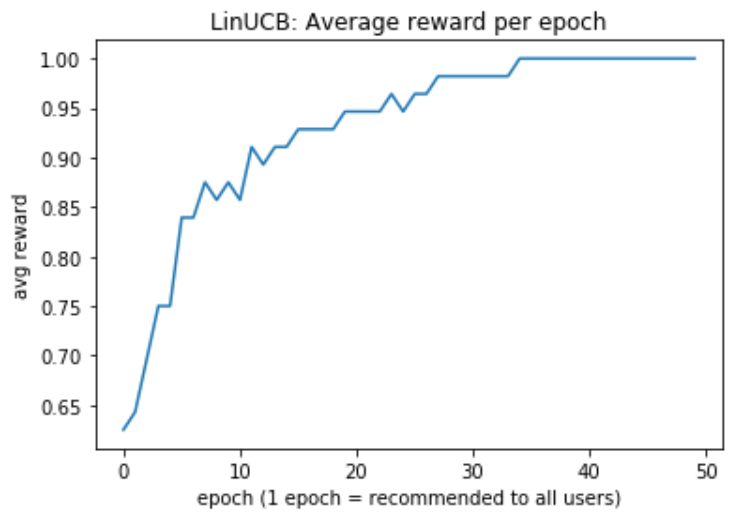
\includegraphics[width=\columnwidth]{img/LinUCB-100items-50epochs}
 \caption{LinUCB trained on 100 items and 56 users for 50 epochs.}
 \label{fig:linUCB}
\end{figure}

\begin{figure}[h]
 \centering
 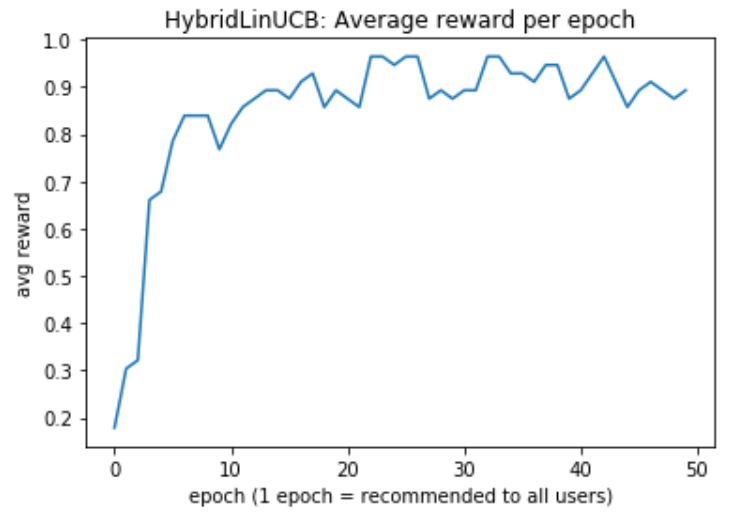
\includegraphics[width=\columnwidth]{img/HybridLinUCB-100items-50epochs}
 \caption{HybridLinUCB trained on 100 items and 56 users for 50 epochs.}
 \label{fig:linUCB}
\end{figure}









\end{document}